\documentclass{beamer}

\usepackage{tikz}
\definecolor{cadet}{rgb}{0.33, 0.41, 0.47}
\definecolor{coolblack}{rgb}{0.0, 0.18, 0.39}

% good resource for themes / colors here:
% http://www.deic.uab.es/~iblanes/beamer_gallery/

\mode<presentation>
{
    \usetheme{Szeged}      % or try Darmstadt, Madrid, Warsaw, ...
    \usecolortheme{seahorse} % or try albatross, beaver, crane, ...
    %\usefonttheme{professionalfonts}  % or try serif, structurebold, ...
    \setbeamertemplate{navigation symbols}{}
    \setbeamertemplate{caption}[numbered]
    \mode<presentation>
    \setbeamercolor*{palette secondary}{use=structure,fg=white,bg=cadet}
    \setbeamercolor*{palette
    tertiary}{use=structure,fg=white,bg=coolblack}
}

\title[Bottom-left title]{An Example Beamer Template}
\author{You!}
\institute{Colorado School of Mines, probably}
\date{\today}

\begin{document}
\begin{frame}
\titlepage
\end{frame}

 \begin{frame}{Test Title}
\begin{itemize}
\item[How] bout
\item Some
\item items?
\end{itemize}
\end{frame}

\section{Background}
\begin{frame}{Pictures!}
\begin{minipage}{\linewidth}
\makebox[\linewidth]{%
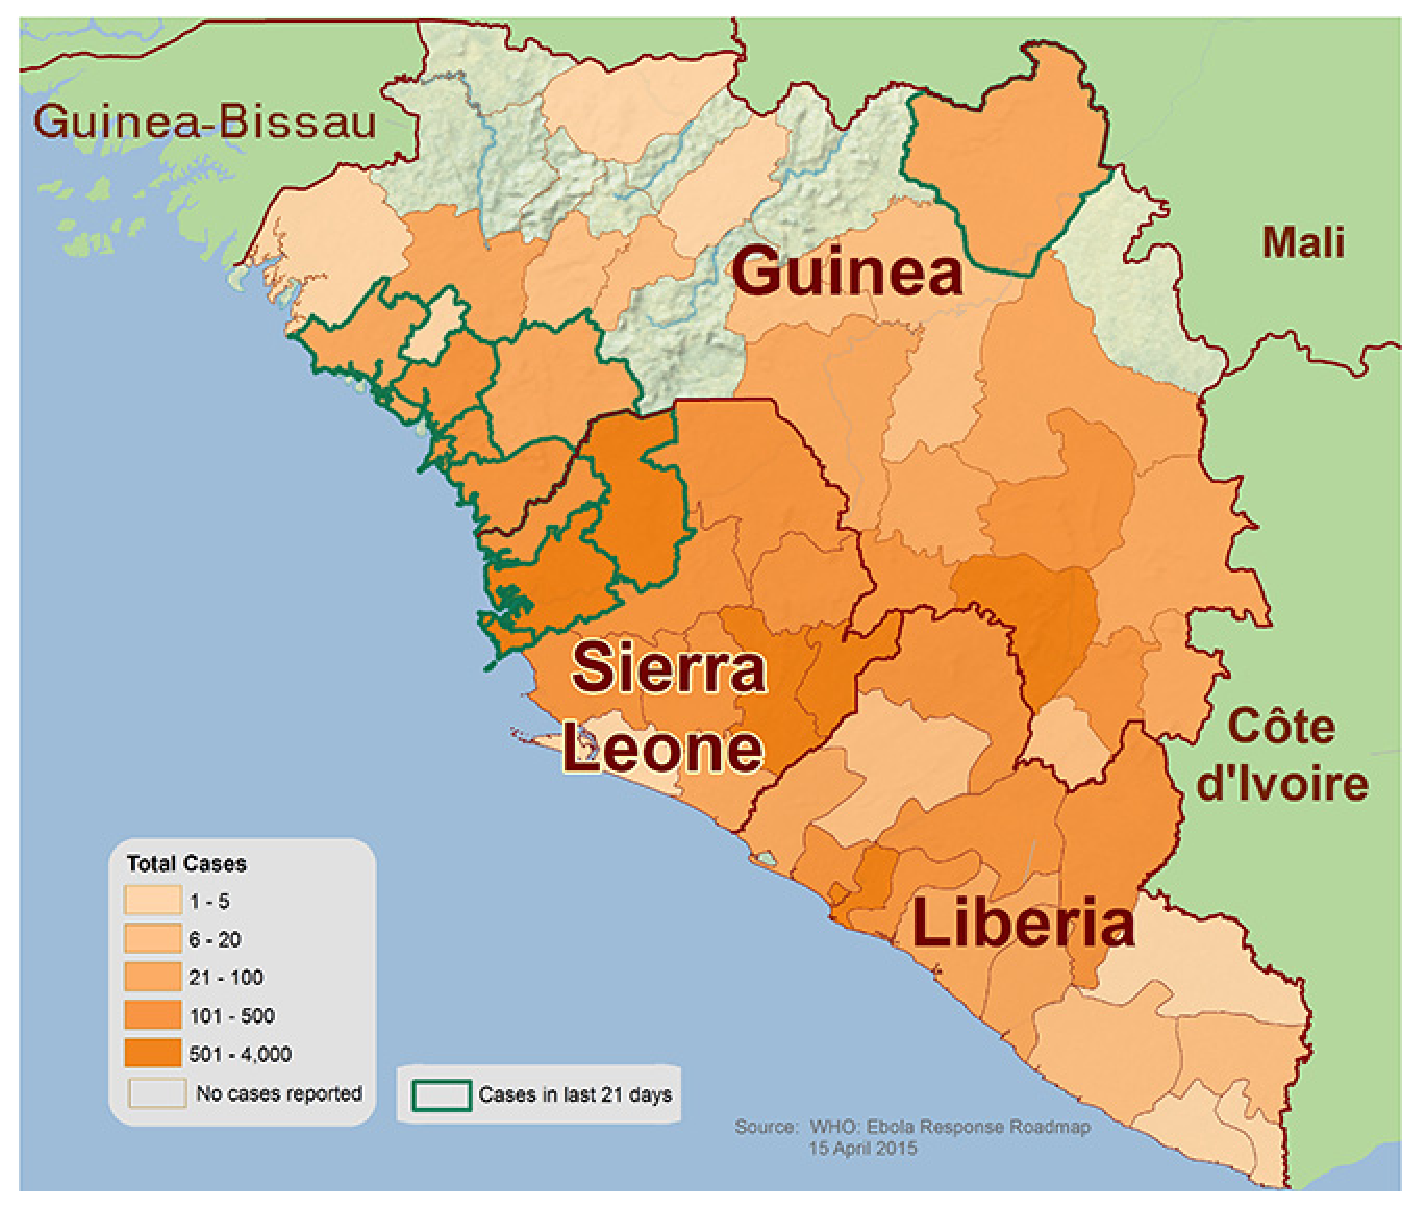
\includegraphics[keepaspectratio=true,scale=0.35]{west-africa-distribution-map.eps}}
\\
\end{minipage}
\end{frame}

\begin{frame}{Columns!}

    \begin{columns} % the "c" option specifies center vertical alignment
        \begin{column}{.6\textwidth} % column designated by a command

        \begin{itemize}
          \item We can have stuff over here
          \item We can choose the size of each column!
        \end{itemize}

        \end{column}
        \begin{column}{.4\textwidth} % column designated by a command

        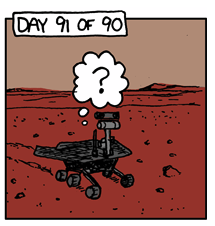
\includegraphics[height=1.5in]{rover.png}

        \end{column}
    \end{columns}

\end{frame}

\begin{frame}{State Diagram}
\tikzstyle{line} = [draw, -latex']
\begin{figure}[ht!]
\begin{center}
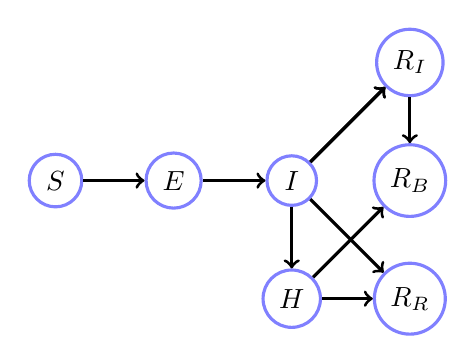
\begin{tikzpicture}[place/.style={circle,draw=blue!50,line width=0.4mm,
fill=white},
transition/.style={->,line width=0.4mm}, scale = 0.5]
\node[place] (s) at (-6, 0) {$S$};
\node[place] (e) at (-3, 0) {$E$};
\node[place] (i) at (0, 0) {$I$};
\node[place] (rb) at (3, 0) {$R_B$};
\node[place](ri) at (3, 3) {$R_I$};
\node[place](rr) at (3, -3) {$R_R$};
\node[place](h) at (0, -3) {$H$};

\path
    (s) edge[transition] node[auto]{} (e)
    (e) edge[transition] node[auto]{} (i)
    (i) edge[transition] node[auto]{} (ri)
    (ri) edge[transition] node[auto]{} (rb)
    (i) edge[transition] node[auto]{} (ri)
    (i) edge[transition] node[auto]{} (rr)
    (i) edge[transition] node[auto]{} (h)
    (h) edge[transition] node[auto]{} (rr)
    (h) edge[transition] node[auto]{} (rb)

;


\end{tikzpicture}
\label{tikz3CM}
\end{center}
\end{figure}


\end{frame}

\section{Example section}
\begin{frame}{Math equations}
\begin{equation*} \left\lbrace
\begin{aligned}
\frac{dS_i}{dt} &= \alpha S_i - \beta_1 S_i I_i -\beta_2 S_i R_{I,i}
-\beta_3S_iH_i\\
\frac{dE_i}{dt} &=  \beta_1 S_i I_i +\beta_2 S_i R_{I,i} +\beta_3S_iH_i-
\delta E_i {\color{red} - \phi_{ij}E_i + \phi_{ji} E_j}\\
\frac{dI_i}{dt} &=  \delta E_i - \gamma_1 I_i-\psi I_i\\
\frac{dH_i}{dt} &= \psi I_i - \gamma_2 H_i \\
\frac{dR_{I,i}}{dt} &= \rho_1\gamma_1 I_i - \omega R_{I,i} \\
\frac{dR_{B,i}}{dt} &= \omega R_{I,i}+\rho_2\gamma_2 H_i \\
\frac{dR_{R,i}}{dt} &= (1-\rho_1)\gamma_1
I_i+(1-\rho_2)\gamma_2 H_i \\%on our notes, we
\end{aligned} \label{std_seir}
\right.
\end{equation*}
\end{frame}

\begin{frame}{Placement Based on Sensitivity Analysis}
Relative change in population steady state given a change in a parameter value
\begin{center}
\begin{tabular}{|c|c|}
\hline
\multicolumn{2}{|c|}{$\displaystyle\frac{\partial \bar{I}}{\partial \psi}\Delta
\psi$} \\
\hline
Guinea & -336.882 \\ \hline
Liberia & -84.6367 \\ \hline
Sierra Leone & -0.467521 \\ \hline
\end{tabular}
\end{center}
\end{frame}

{\setbeamercolor{background canvas}{bg=cadet}
\begin{frame}
\centering \Huge \color{white} Questions?

\end{frame}}

\begin{frame}{References}

\begin{thebibliography}{3}
\setbeamertemplate{bibliography item}[text]
\tiny
\bibitem{cdc} Center for Disease Control. \emph{Questions and Answers:
Estimating the Future Number of Cases in the Ebola Epidemic}, 2015.

\bibitem{dynamics}J. Lewnard et. al. \emph{Dynamics and Control of Ebola virus
Transmission in Montserrado, Liberia: a mathematical modeling analysis}
Department of Epidemiology of Microbial Diseases. Yale,
CT. Dec 2014.
ttt{http://www.cdc.gov/vhf/ebola/outbreaks/2014-west-africa/qa-mmwr-estimating-future-cases.html}

\bibitem{WorldBank} ``Population Growth (annual \%)." The World Bank. Web. 26
Mar. 2015. http://data.worldbank.org/indicator/SP.POP.GROW.


\end{thebibliography}

\end{frame}
\end{document}
